% !TEX root = ../main.tex

\chapter{Background and Validation of the FW-H Method} \label{sec:derivations}

In this chapter, the FW-H method as well as the analytical methods by which it is validated are described. The formulation used in the numerical FW-H method is described in Section \ref{sec:FWH_desc} below along with the description of how the computer code works. The following sections will then describe the test cases used to validate the code; describe the analytical solutions of the monopole and dipole used to compare against the numerical solution; and finally, the validation data is presented to build confidence in the numerical code itself.

\section{Description of the FW-H Method}\label{sec:FWH_desc}
\subsection{Derivation of the FW-H Equation}\label{subsec:FWH_derivation}

To predict the open rotor noise, the FW-H equation in its permeable surface form provides a useful basis for noise prediction. This formulation is based on the governing laws of fluid motion, and the descriptions provided below are based on the original paper by Ffowcs Williams and Hawkings \cite{FfowcsWilliams1969}. Consider a control surface \textit{S}, in which contains a combination of fluid and solid boundaries, while the region outside contains only fluid. \textit{S} moves with a velocity $v$ and is defined by the equation $f(x,t)=0$, the following relationship then hold

\begin{gather}
    f < 0, H(f) = 0 \nonumber \\
    f > 0, H(f) = 1 \nonumber \\
    \nabla_x f = |\nabla_x f|\textbf{n}, \text{\textbf{n} is the outward normal to } S \\
    D_v f /Dt = 0, \text{ so } \partial f / \partial t = -v_{\textbf{n}}|\nabla_x f| \nonumber \\
    \partial H(f) / \partial x_i = \delta(f) \partial f / \partial x_i = \delta(f)\textbf{n}_i|\nabla_x f| \nonumber
\end{gather}

\begin{figure}[H]
    \centering
    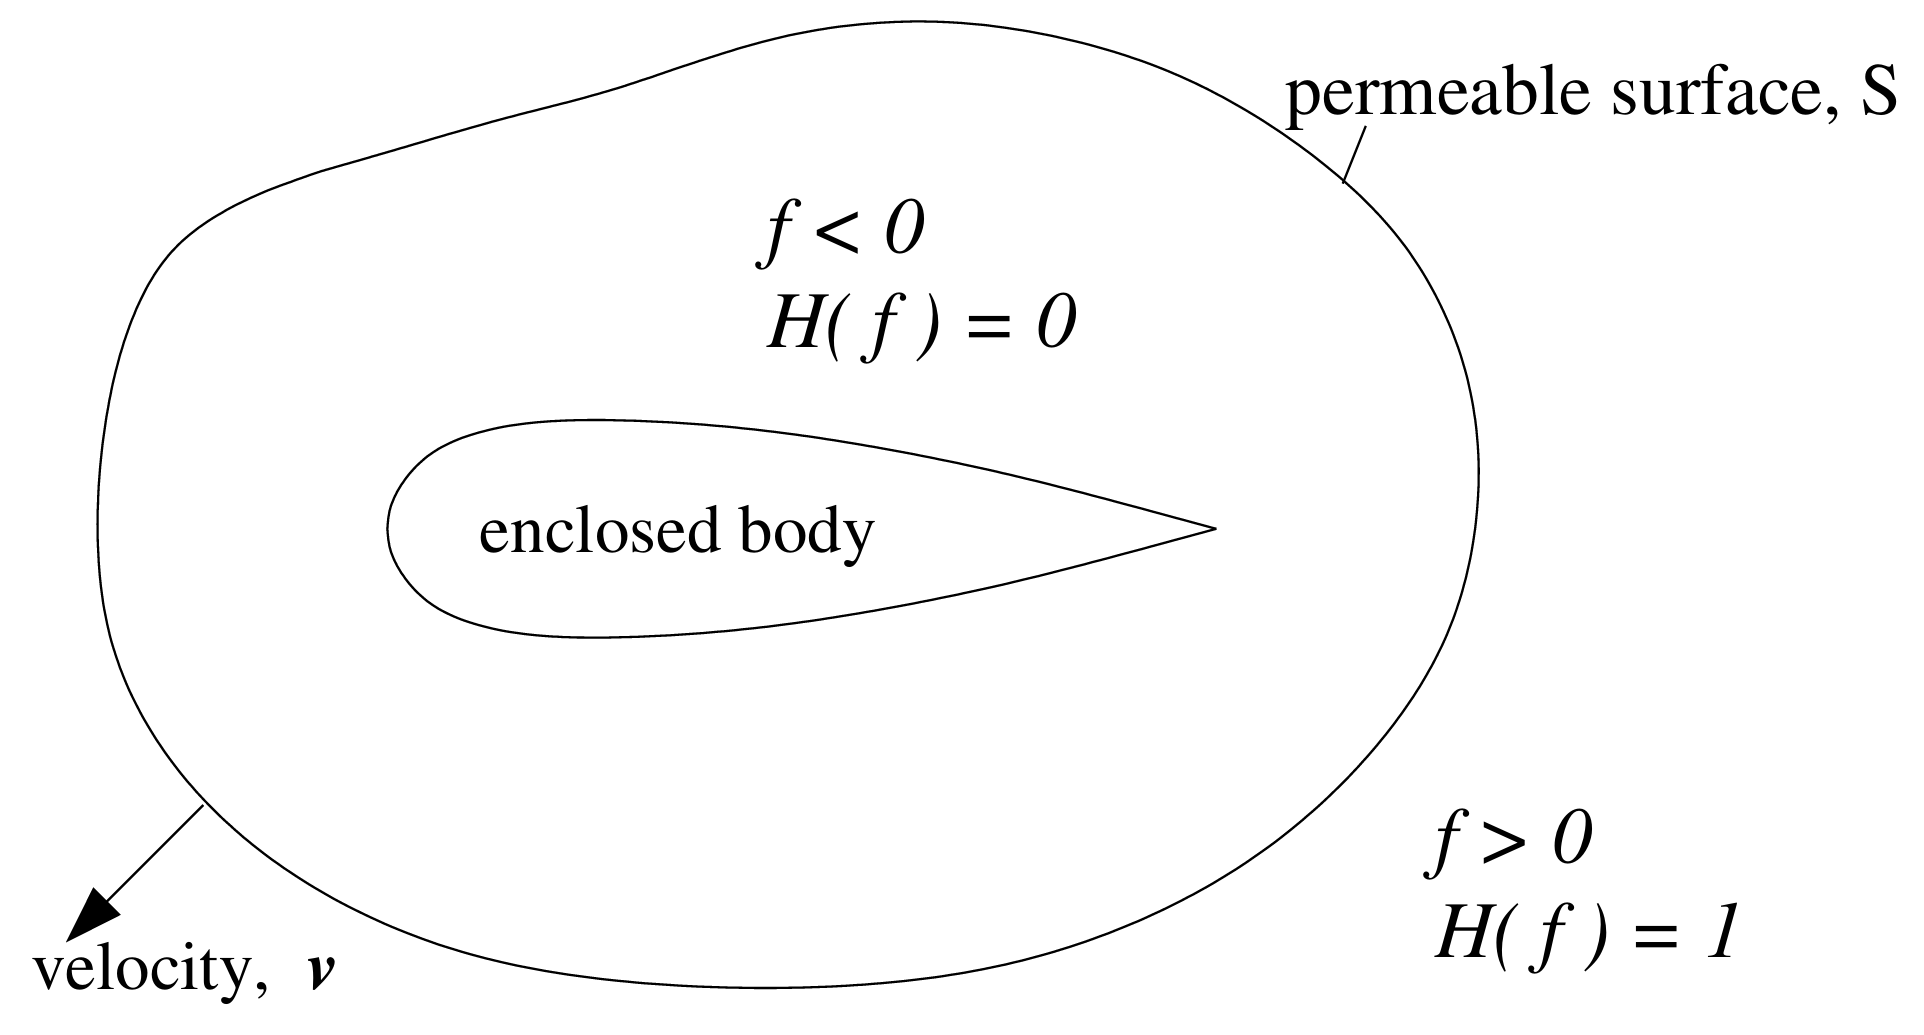
\includegraphics[width=0.5\linewidth]{fig_misc/heaviside.png}
    \caption{Permeable control surface}
    \label{fig:heaviside}
\end{figure}

Generalised flow variables are denoted by an overbar. Outside of the surface, the variables are equal to the real flow variables, while inside they are assigned the value zero, hence are discontinuous acorss \textit{S}. Manipulating the mass and momentum conservation equations,

\begin{equation}
    \begin{gathered}
        H(f)\left(\frac{\partial \rho'}{\partial t} + \frac{\partial \rho u_i}{\partial x_i}\right) = 0 \\
        \frac{\partial \overline{\rho'}}{\partial t} + \frac{\partial (\overline{\rho u_i})}{\partial x_i} = (\rho_0 u_{\textbf{n}} + \rho'(u_{\textbf{n}} - v_{\textbf{n}}))\delta(f)|\nabla_x f|
    \end{gathered}
    \label{eq:continuity_heaviside}
\end{equation}

\begin{equation}
    \begin{gathered}
        H(f)\left(\frac{\partial (\rho u_i)}{\partial t} + \frac{\partial}{\partial x_j}(p_{ij} + \rho u_i u_j)\right) = 0 \\
        \frac{\partial (\overline{\rho u_i})}{\partial t} + \frac{\partial}{\partial x_j}(\overline{p_{ij}} + \overline{\rho u_i u_j}) = (p_{ij}\textbf{n}_j + \rho u_i (u_{\textbf{n}} - v_{\textbf{n}})) \delta(f) |\nabla_x f|
    \end{gathered}
    \label{eq:momentum_heaviside}
\end{equation}

subtracting the divergence \ref{eq:momentum_heaviside} from the time derivative \ref{eq:continuity_heaviside} gives an inhomogeneous wave equation,

\begin{equation}
    \begin{split}
        \Box^2 p'(x,t) &= \frac{\partial^2 \overline{T_{ij}}}{\partial x_i \partial x_j} - \frac{\partial}{\partial x_i} \left(p_{ij}\textbf{n}_j + \rho u_i (u_{\textbf{n}} - v_{\textbf{n}}) \right) \delta(f) |\nabla_x f| \\
        &\quad + \frac{\partial}{\partial t} \left(\rho_0 u_{\textbf{n}} + \rho'(u_{\textbf{n}} - v_{\textbf{n}}) \right) \delta(f) |\nabla_x f| 
    \end{split}
    \label{eq:FWH_diff}
\end{equation}

Which is the differential form of the FW-H equation, and is the equation governing the generation and propagation of sound. Converting this differential form into an equivalent integral form is done using Green's function. A coordinate change from the fixed one to a moving one with the control surface $\eta$ is performed so the sources are at rest in the $\eta$ space. The Jacobian for the coordinate change is $J$ which represents the ratio of volume elements in the $\eta$ and $y$ spaces. Performing the steps above gives the inhomogeneous wave equation in the integral form of the FW-H equation,

\begin{equation}
    \begin{split}
        p'(\bm{x},t) &=
        \frac{\partial^2}{\partial x_i\partial x_j} \int_{-\infty}^{\infty} \frac{\overline{T_{ij}}\delta(g)J}{4\pi r}d^3\eta d\tau \\
        &\quad - \frac{\partial}{\partial x_i} \int_{-\infty}^\infty \frac{\left(p_{ij}\textbf{n}_j+\rho u_i (u_{\textbf{n}}-v_{\textbf{n}}) \right) \delta(f)\delta(g) |\nabla_xf|J}{4\pi r} d^3\eta d\tau \\
        &\quad + \frac{\partial}{\partial t} \int_{-\infty}^\infty \frac{\left(\rho_0u_{\textbf{n}} + \rho'(u_{\textbf{n}}-v_{\textbf{n}}) \right) \delta(f)\delta(g) |\nabla_xf|J}{4\pi r}d^3\eta d\tau
    \end{split}
    \label{eq:FWH}
\end{equation}

The first RHS term, the quadrupole, is not dealt with explicitly \cite{Parry1988, Hanson1985} as it is more significant for transonic and supersonic Mach numbers \cite{FfowcsWilliams1969, Ffowcs1969}. By choosing a sufficiently large permeable surface, the quadrupole contributions outside of this surface is negligible,

\begin{equation}
    \begin{split}
        p'(\bm{x},t) &=
        - \frac{\partial}{\partial x_i} \int_{-\infty}^\infty \frac{\left(p_{ij}\textbf{n}_j+\rho u_i (u_{\textbf{n}}-v_{\textbf{n}}) \right) \delta(f)\delta(g) |\nabla_xf|J}{4\pi r} d^3\eta d\tau \\
        &\quad + \frac{\partial}{\partial t} \int_{-\infty}^\infty \frac{\left(\rho_0u_{\textbf{n}} + \rho'(u_{\textbf{n}}-v_{\textbf{n}}) \right) \delta(f)\delta(g) |\nabla_xf|J}{4\pi r}d^3\eta d\tau
    \end{split}
    \label{eq:FWH_no_quad}
\end{equation}

 Using the notation by di Francescantonio \cite{Francescantonio1997} to simplify the algebra, new variables $U_i$ and $L_i$ are introduced to represent mass and momentum fluxes through the control surface,

\begin{equation*}
    U_i=(1-\frac{\rho}{\rho_0})v_i  + \frac{\rho}{\rho_0}u_i \quad     
    L_i=p_{ij}\textbf{n}_j+pu_i(u_{\textbf{n}}-v_{\textbf{n}})
\end{equation*}

Considering an undistorted control surface that translates at a constant and subsonic velocity, the retarded time formulation, as described by Brentner and Farassat \cite{Brentner1998} is,

\begin{equation}
\begin{split}
    p'(\bm{x}, t) 
    &= \frac{1}{4\pi} \int_{S} \left[ \frac{\rho_0 (\dot{U}_{\textbf{n}} + U_{\hat{\textbf{n}}})}{r(1-M_r)^2} \right]_{\tau^*} dS(\eta) \\
    &\quad + \frac{1}{4\pi} \int_{S} \left[ \frac{\rho_0 (r(dM/d\tau)_r + c(M_r - |M|^2))}{r^2(1-M_r)^3} \right]_{\tau^*} dS(\eta) \\
    &\quad + \frac{1}{4\pi c} \int_{S} \left[ \frac{\dot{L}_r}{r(1-M_r)^2} \right]_{\tau^*} dS(\eta) \\
    &\quad + \frac{1}{4\pi} \int_{S} \left[ \frac{L_r - L_m}{r^2(1-M_r)^2} \right]_{\tau^*} dS(\eta) \\
    &\quad + \frac{1}{4\pi c} \int_{S} \left[ \frac{L_r(r(dM/d\tau)_r + c(M_r - |M|^2))}{r^2(1-M_r)^3} \right]_{\tau^*} dS(\eta)
\end{split}
\label{eq:fwh_full_expansion}
\end{equation}

The retarded time are calculated implicitly via the Newton-Raphson root-finding method. 

\subsection{Description of the FW-H Code} \label{subsec:FWH_description}
The FW-H code was written in Fortran 90 to implement the calculations computationally using equation \ref{eq:fwh_full_expansion}. The program is summarised in the figure below,

\begin{figure}[H]
    \centering
    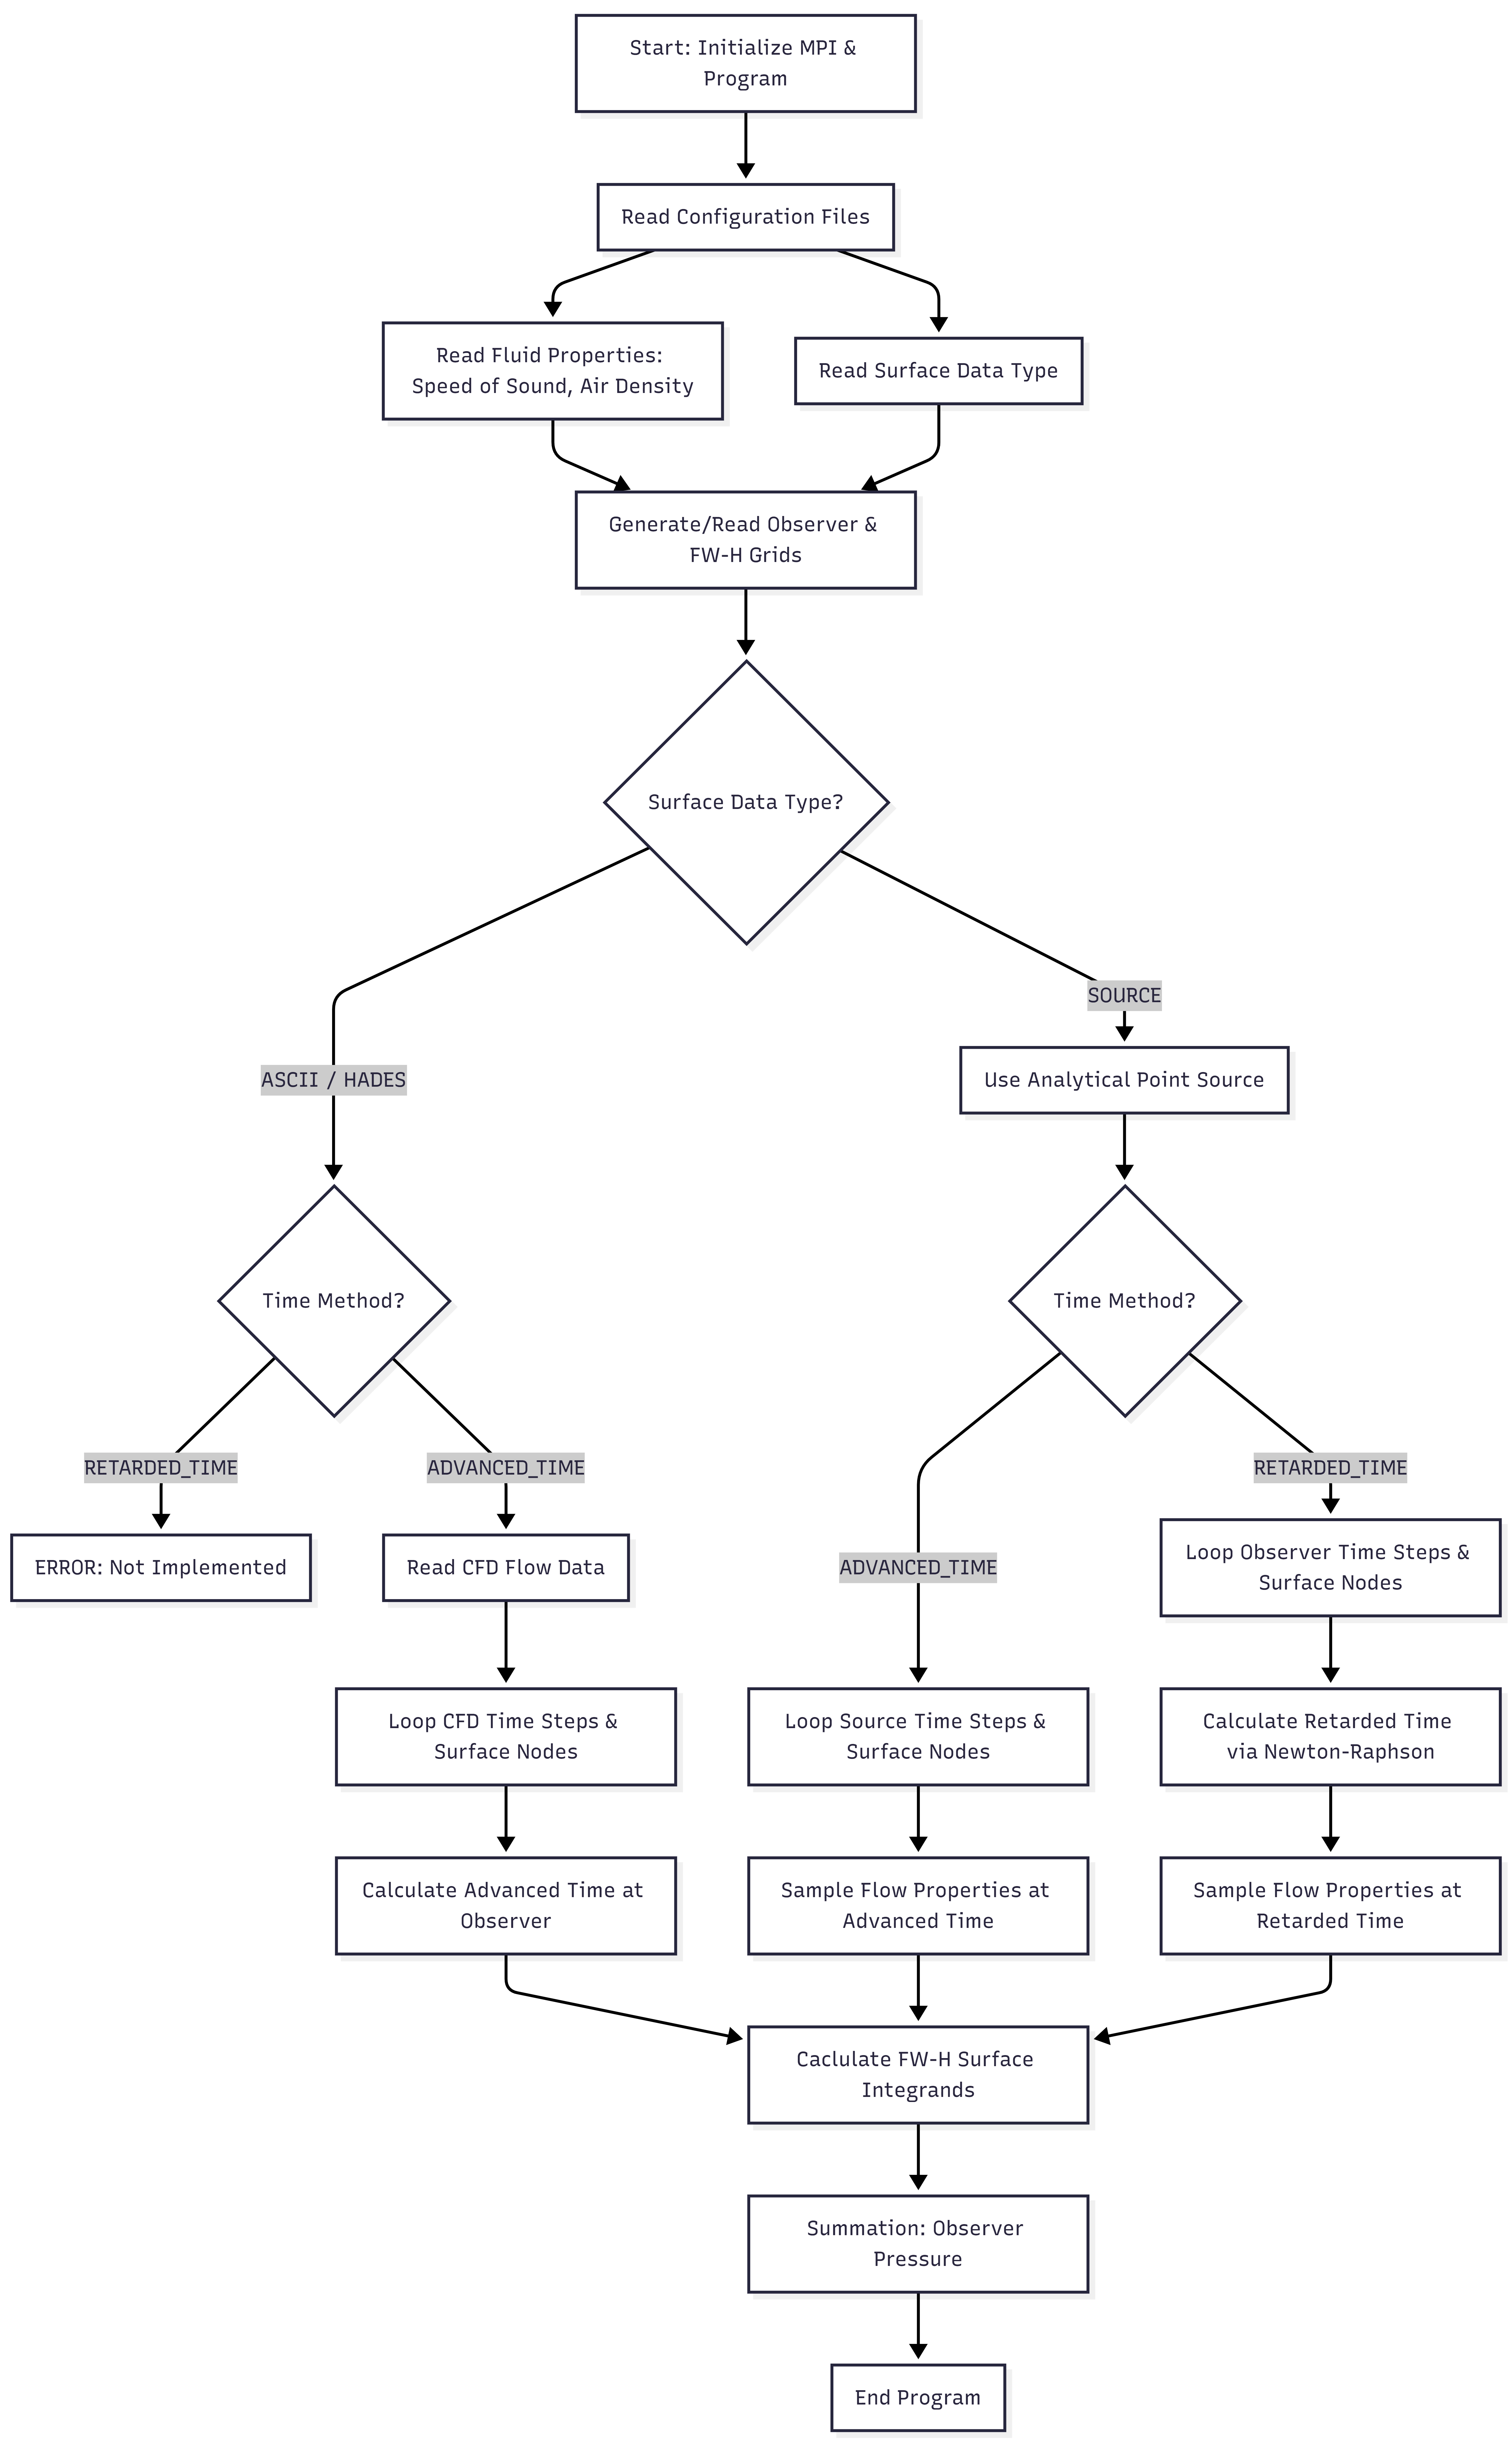
\includegraphics[width=0.7\linewidth]{fig_misc/FWH_Flowchart.png}
    \label{fig:fwh_flowchart}
\end{figure}

The ambient flow properties are first defined to be used as reference values. The code then checks whether the input is 'Source' or 'ASCII/HADES'; the former uses the analytical point source that will be described in the following sections, and the latter uses CFD data as input and uses its grid

\section{Validation of the FW-H Code} \label{sec:validation_description}
To compare the accuracy of the derivations described in Chapter \ref{sec:derivations}, several test cases are used to model a point sound source and an observer. This section describes the test cases used and the validations. Figure \ref{fig:fwh_validation} below illustrates the framework used for validation. 

\begin{figure}[H]
    \centering
    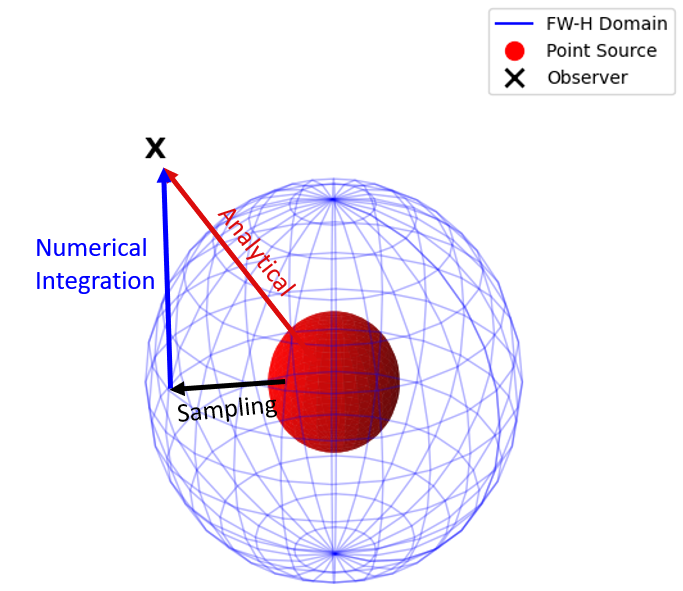
\includegraphics[width=0.5\linewidth]{fig_monopole/fwh_domain_observer_arrows.png}
    \caption{Code validation framework}
    \label{fig:fwh_validation}
\end{figure}

The numerical code samples the source to the permeable boundary (black arrow), followed by surface integration of pressure to calculate the acoustic pressure at the observer (blue arrow). Analytical pressure is calculated directly from the source to the observer (red arrow).

\subsection{Test Cases} \label{subsubsec:test_cases}
In all validation test cases, the point source is prescribed with strength $Q(\tau)=\sin{(10\tau)}$, from a starting point at the origin, $\left[0,0,0\right]$. Speed of sound $c$ and freestream density $\rho_0$ are set to $340m/s$ and $1.2 kg/m^3$, respectively. The observer's location depends on the case. A control surface surrounding the source are prescribed with a radius $r$. 

These following are based on the work of Char \cite{TingChar2024} and are extended for dipoles:

\begin{itemize}
    \item Stationary and co-translating point source and observer. This test case is used as a baseline to test the overall prediction of the zero relative motion between point source and observer. The tests will also demonstrate the similarity between the two cases. 
    
    \begin{figure}[H]
        \begin{subfigure}[b]{0.495\textwidth}
            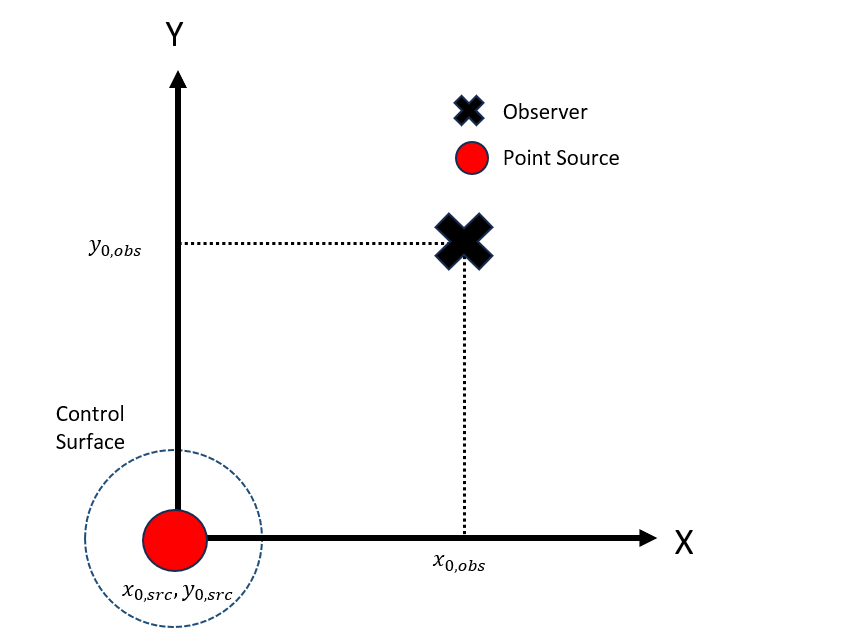
\includegraphics[width=\textwidth]{fig_test_cases/stationary_stationary.png}
            \caption{}
            \label{fig:testcase_ss}
        \end{subfigure}
        \hfill
        \begin{subfigure}[b]{0.495\textwidth}
            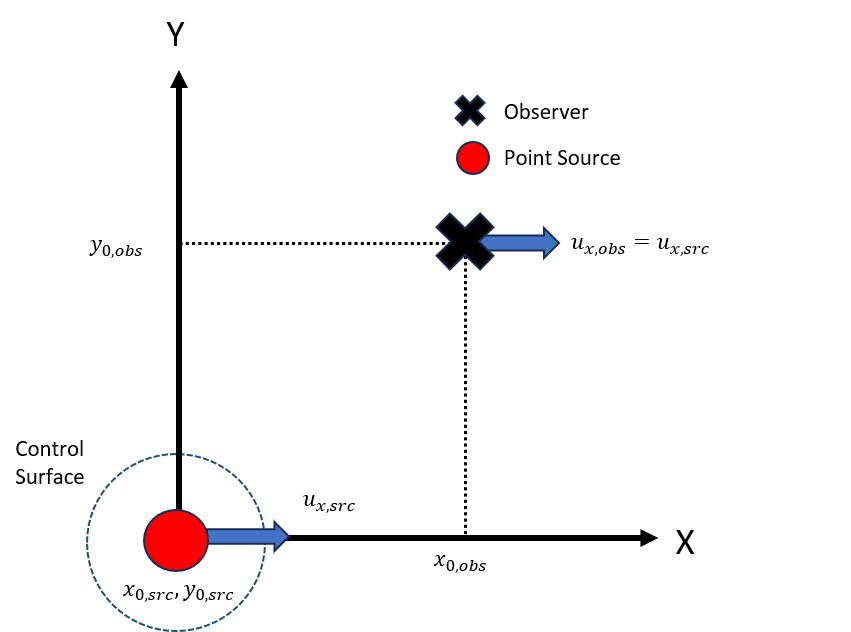
\includegraphics[width=\textwidth]{fig_test_cases/translating_translating.png}
            \caption{}
            \label{fig:testcase_tt}
        \end{subfigure}
        \caption{\centering Illustration of, a) stationary point source and observer, and b) co-translating point source and observer cases}
        \label{fig:testcase_ss_tt}
    \end{figure}
    
    \item Translating point source and stationary observer. This test case demonstrates the prediction with cases of non-zero relative motion between point source and observer, and thus shows the limitations of some of the derivations.
    
    \begin{figure}[H]
        \centering
        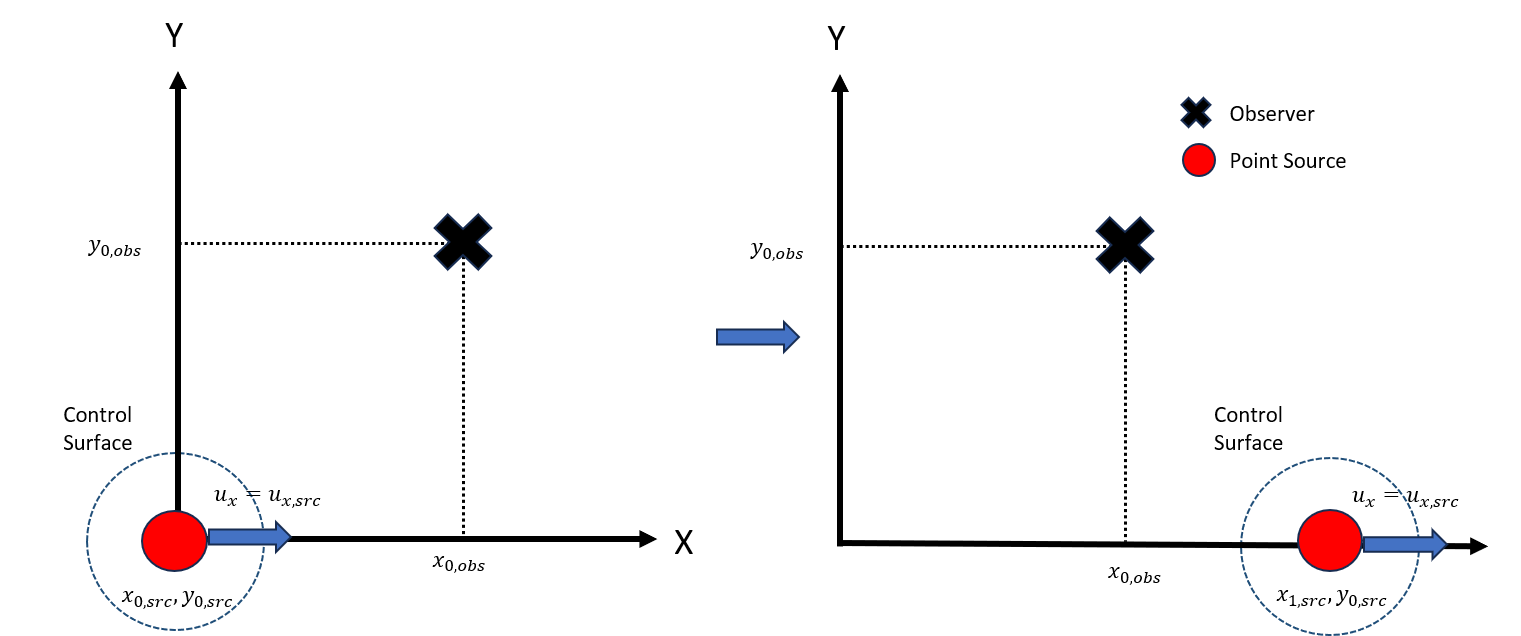
\includegraphics[width=1\linewidth]{fig_test_cases/translating_stationary.png}
        \caption{Illustration of translating point source and stationary observer cases}
        \label{fig:testcase_ts}
    \end{figure}
    
\end{itemize}

Any error are then be quantified using the following,

\begin{equation}
    Error = \frac{\Sigma_j(p_{j,ref} - p_{j,num})^2}{\Sigma_j(p^j_{ref})^2} 
    \label{eq:error}
\end{equation}

\clearpage
% where the subscripts $j$, $ref$, and $num$ are the $j$-th index, reference analytical values, and the numerical integration results, respectively. 